% begin module rolles-theorem
\begin{frame}[t]
\begin{theorem}[Rolle's Theorem]
Let $f$ be a function that satisfies the following three conditions:
\begin{itemize}
\item  $f$ is continuous on the closed interval $[a,b]$.
\item  $f$ is differentiable on the open interval $(a,b)$.
\item  $f(a) = f(b)$.
\end{itemize}
Then there is a number $c$ in $(a,b)$ such that $f'(c) = 0$.
\end{theorem}
\begin{columns}[c]
\column{.3\textwidth}
\uncover<3->{%
\ \only<handout:1| -3>{%

\psset{xunit=0.7cm, yunit=0.7cm}
\begin{pspicture}(-5, -5)(5,5)
\psframe*[linecolor=white](-5,-5)(5,5)
\psaxes[ticks=none, labels=none]{<->}(0,0)(-0.5,-0.5)(4.5,2.5)
\psline[linecolor=red](0.5, 1.5)(4, 1.5)
\psline[linestyle=dashed](1, 0)(1, 1.5)
\psline[linestyle=dashed](3.5, 0)(3.5, 1.5)
\fcFullDot{0.5}{1.5}
\fcFullDot{4}{1.5}
\tiny
\rput[t](0.5, -0.1){$a$}
\rput[t](1, -0.1){$c_1$}
\rput[t](3.5, -0.1){$c_2$}
\rput[t](4, -0.1){$b$}
\psline(0.5, 0)(0.5, 0.1)
\psline(4, 0)(4, 0.1)
\end{pspicture}
%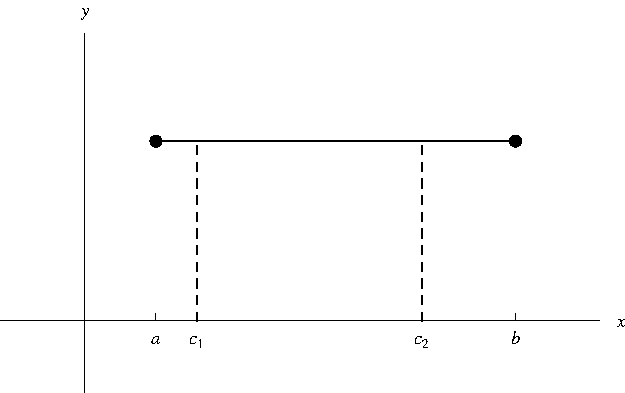
\includegraphics[height=2.2cm]{maxima-minima/pictures/04-02-rollesa.pdf}%
}%
}%
\only<handout:2-3| 4->{%
\psset{xunit=0.7cm, yunit=0.7cm}
\begin{pspicture}(-5, -5)(5,5)
\psframe*[linecolor=white](-5,-5)(5,5)
\psaxes[ticks=none, labels=none]{<->}(0,0)(-0.5,-0.5)(5,2.5)
\fcFullDot{0.5}{1.61458}
\fcFullDot{4.6711646096}{1.61458}
\tiny
\rput[t](0.5, -0.1){$a$}
\rput[t](1, -0.1){$c_1$}
\rput[t](3.5, -0.1){$c_2$}
\rput[t](4.6711646096, -0.1){$b$}
\psline(0.5, 0)(0.5, 0.1)
\psline(4.6711646096, 0)(4.6711646096, 0.1)
%Function formula: -9/8 ((x)^{2})+1/6 ((x)^{3})+1+7/4 (x)
\psplot[linecolor=red, plotpoints=1000]{0.5}{4.6711646096}{x 1.75 mul 1 add x 3 exp 0.166667 mul add x 2 exp -1.125 mul add }
\psline[linestyle=dashed](1, 0)(1, 1.79167)
\psline[linestyle=dashed](3.5, 0)(3.5, 0.489583)
\fcFullDotBlue{1}{1.79167}
\psline[linecolor=blue]( 0.5, 1.79167)(1.5, 1.79167)
\fcFullDotBlue{3.5}{0.489583}
\psline[linecolor=blue]( 3,0.489583)(4, 0.489583)
\end{pspicture}
%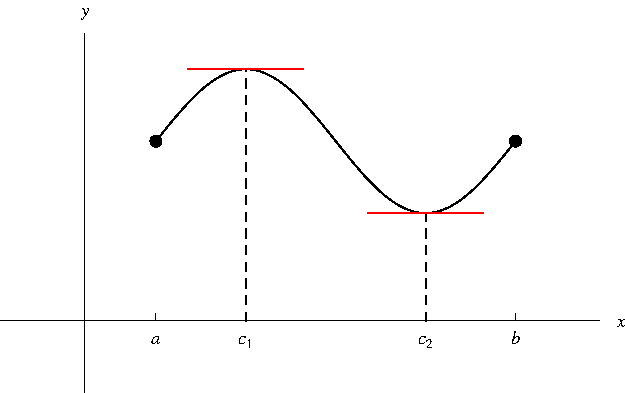
\includegraphics[height=2.2cm]{maxima-minima/pictures/04-02-rollesc.pdf}%
}%

\uncover<handout:2| 4->{%
\only<handout:-2| -4>{%
\psset{xunit=0.7cm, yunit=0.7cm}
\begin{pspicture}(-5, -5)(5,5)
\psframe*[linecolor=white](-5,-5)(5,5)
\psaxes[ticks=none, labels=none]{<->}(0,0)(-0.5,-0.5)(5,2.5)
\fcFullDot{0.5}{1.77083}
\fcFullDot{4.67116}{1.77083}
\tiny
\rput[t](0.5, -0.1){$a$}
\rput[t](4.67116, -0.1){$b$}
\psline(0.5, 0)(0.5, 0.1)
\psline(4.67116, 0)(4.67116, 0.1)
%Function formula: -1/12 ((3932720999/20855823048+6495190525/10427911524 (x))^{3})+1/8 ((3932720999/20855823048+6495190525/10427911524 (x))^{2})+66500190143/41711646096+6495190525/20855823048 (x)
\psplot[linecolor=red, plotpoints=1000]{0.5}{4.67116}{x 0.311433 mul 1.59428 add x 0.622866 mul 0.188567 add 2 exp 0.125 mul add x 0.622866 mul 0.188567 add 3 exp -0.0833333 mul add }
\rput[t](2.90822, -0.1){$c$}
\psline[linestyle=dashed](2.90822, 0)(2.90822, 2.33333)
\fcFullDotBlue{2.90822}{ 2.33333}
\psline[linecolor=blue]( 2.40822, 2.33333)(3.40822,  2.33333)
\end{pspicture}
%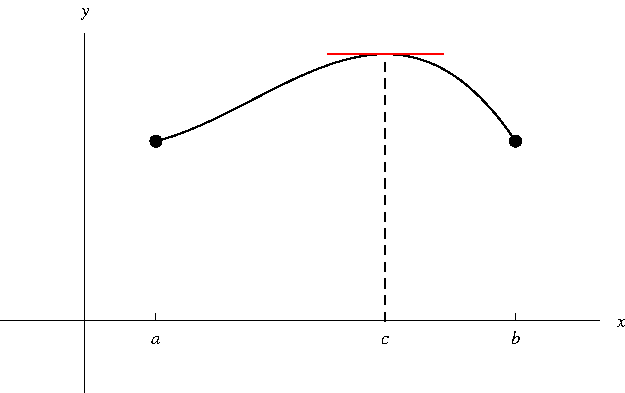
\includegraphics[height=2.2cm]{maxima-minima/pictures/04-02-rollesb.pdf}%
}%
}%
\only<handout:3| 5->{%
\psset{xunit=0.7cm, yunit=0.7cm}
\begin{pspicture}(-5, -5)(5,5)
\psframe*[linecolor=white](-5,-5)(5,5)
\psaxes[ticks=none, labels=none]{<->}(0,0)(-0.5,-0.5)(5,2.5)
\fcFullDot{0.5}{2.31944}
\fcFullDot{4.67116}{2.31944}
\tiny
\rput[t](0.5, -0.1){$a$}
\rput[t](4.67116, -0.1){$b$}
\psline(0.5, 0)(0.5, 0.1)
\psline(4.67116, 0)(4.67116, 0.1)
%Function formula: -10405359841/11250000000 (x)-1/12 ((x)^{2})+62905359841/22500000000+1/18 ((x)^{3})
\psplot[linecolor=red, plotpoints=1000]{0.5}{4.67116}{x 3 exp 0.0555556 mul 2.79579 add x 2 exp -0.0833333 mul add x -0.924921 mul add }
\rput[t](2.90822, -0.1){$c$}
\psline[linestyle=dashed](2.90822, 0)(2.90822,0.767607)
\fcFullDotBlue{2.90822}{ 0.767607}
\psline[linecolor=blue]( 2.40822, 0.767607)(3.40822, 0.767607)
\end{pspicture}
%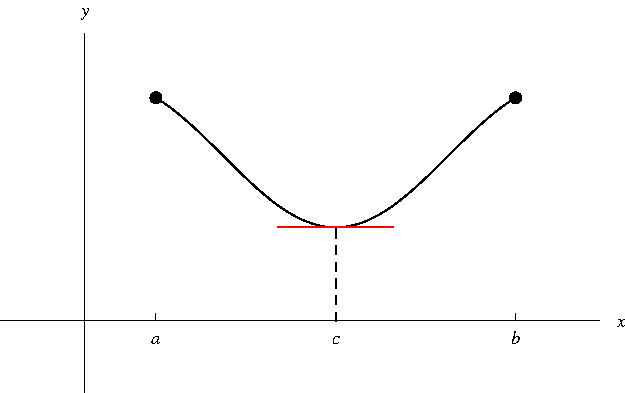
\includegraphics[height=2.2cm]{maxima-minima/pictures/04-02-rollesd.pdf}%
}%
\column{.6\textwidth}
\uncover<2->{%
The proof breaks down into three cases:
\begin{enumerate}
\item<1-| alert@3>  \alert<handout:1| 0>{$f$ is a horizontal line.}
\item<1-| alert@4>  \alert<handout:2| 0>{$f(x) > f(a)$ for some $x$ in $(a,b)$.}
\item<1-| alert@5>  \alert<handout:3| 0>{$f(x) < f(a)$ for some $x$ in $(a,b)$.}
\end{enumerate}
}%
\end{columns}

\vspace{2cm} %guarantees top alignment of slide
\end{frame}


\begin{frame}[t]
\begin{theorem}[Rolle's Theorem]
Let $f$ be a function that satisfies the following three conditions:
\begin{itemize}
\item  $f$ is continuous on the closed interval $[a,b]$.
\item  $f$ is differentiable on the open interval $(a,b)$.
\item  $f(a) = f(b)$.
\end{itemize}
Then there is a number $c$ in $(a,b)$ such that $f'(c) = 0$.
\end{theorem}
\begin{proof}
\begin{columns}[c]
\column{.3\textwidth}
\psset{xunit=0.7cm, yunit=0.7cm}
\begin{pspicture}(-5, -5)(5,5)
\psframe*[linecolor=white](-5,-5)(5,5)
\psaxes[ticks=none, labels=none]{<->}(0,0)(-0.5,-0.5)(4.5,2.5)
\psline[linecolor=red](0.5, 1.5)(4, 1.5)
\psline[linestyle=dashed](1, 0)(1, 1.5)
\psline[linestyle=dashed](3.5, 0)(3.5, 1.5)
\fcFullDot{0.5}{1.5}
\fcFullDot{4}{1.5}
\tiny
\rput[t](0.5, -0.1){$a$}
\rput[t](1, -0.1){$c_1$}
\rput[t](3.5, -0.1){$c_2$}
\rput[t](4, -0.1){$b$}
\psline(0.5, 0)(0.5, 0.1)
\psline(4, 0)(4, 0.1)
\end{pspicture}
%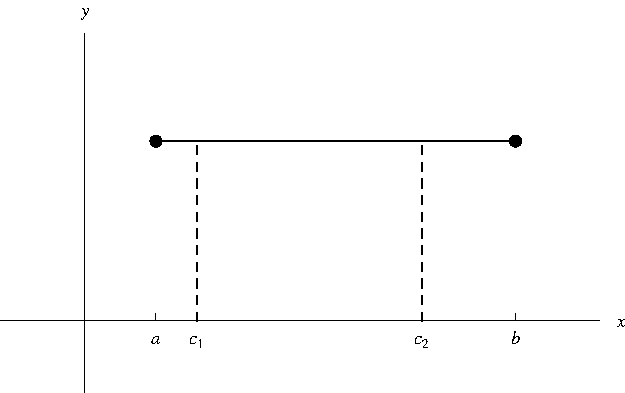
\includegraphics[height=2.5cm]{maxima-minima/pictures/04-02-rollesa.pdf}%
\column{.6\textwidth}
\begin{enumerate}
\item  $f$ is a horizontal line.
\end{enumerate}
\begin{itemize}
\item<2->  Then \alert<handout:0| 2-3>{$f'(x) = \uncover<3->{0.}$}
\item<4->  Therefore we can take $c$ to be any number in $(a,b)$. \qedhere
\end{itemize}
\end{columns}
\end{proof}

\vspace{2cm} %guarantees top alignment of slide
\end{frame}


\begin{frame}[t]
\begin{theorem}[Rolle's Theorem]
Let $f$ be a function that satisfies the following three conditions:
\begin{itemize}
\item  $f$ is continuous on the closed interval $[a,b]$.
\item<1-| alert@4>  $f$ is differentiable on the open interval $(a,b)$.
\item<1-| alert@3>  $f(a) = f(b)$.
\end{itemize}
Then there is a number $c$ in $(a,b)$ such that $f'(c) = 0$.
\end{theorem}
\begin{proof}
\begin{columns}[c]
\column{.3\textwidth}
\psset{xunit=0.7cm, yunit=0.7cm}
\begin{pspicture}(-5, -5)(5,5)
\psframe*[linecolor=white](-5,-5)(5,5)
\psaxes[ticks=none, labels=none]{<->}(0,0)(-0.5,-0.5)(5,2.5)
\fcFullDot{0.5}{1.77083}
\fcFullDot{4.67116}{1.77083}
\tiny
\rput[t](0.5, -0.1){$a$}
\rput[t](4.67116, -0.1){$b$}
\psline(0.5, 0)(0.5, 0.1)
\psline(4.67116, 0)(4.67116, 0.1)
%Function formula: -1/12 ((3932720999/20855823048+6495190525/10427911524 (x))^{3})+1/8 ((3932720999/20855823048+6495190525/10427911524 (x))^{2})+66500190143/41711646096+6495190525/20855823048 (x)
\psplot[linecolor=red, plotpoints=1000]{0.5}{4.67116}{x 0.311433 mul 1.59428 add x 0.622866 mul 0.188567 add 2 exp 0.125 mul add x 0.622866 mul 0.188567 add 3 exp -0.0833333 mul add }
\rput[t](2.90822, -0.1){$c$}
\psline[linestyle=dashed](2.90822, 0)(2.90822, 2.33333)
\fcFullDotBlue{2.90822}{ 2.33333}
\psline[linecolor=blue]( 2.40822, 2.33333)(3.40822,  2.33333)
\end{pspicture}
%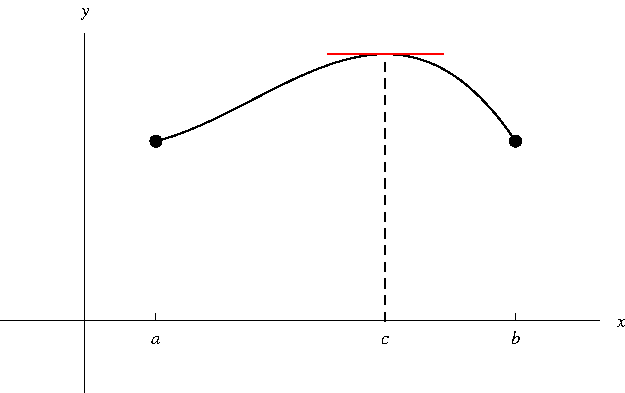
\includegraphics[height=2.5cm]{maxima-minima/pictures/04-02-rollesb.pdf}%
\column{.6\textwidth}
\begin{enumerate}
\setcounter{enumi}{1}
\item  $f(x) > f(a)$ for some $x$ in $(a,b)$.
\end{enumerate}
\begin{itemize}
\item<2->  By the Extreme Value Theorem, $f$ has a maximum in $[a,b]$.
\item<3->  Since $f(x) > f(a)$, this value is attained at some $c$ in $(a,b)$.
\item<4->  \alert<handout:0| 4>{Fermat's Theorem}: $f'(c) = 0$.\qedhere
\end{itemize}
\end{columns}
\end{proof}

\vspace{2cm} %guarantees top alignment of slide
\end{frame}



\begin{frame}[t]
\begin{theorem}[Rolle's Theorem]
Let $f$ be a function that satisfies the following three conditions:
\begin{itemize}
\item  $f$ is continuous on the closed interval $[a,b]$.
\item<1-| alert@4>  $f$ is differentiable on the open interval $(a,b)$.
\item<1-| alert@3>  $f(a) = f(b)$.
\end{itemize}
Then there is a number $c$ in $(a,b)$ such that $f'(c) = 0$.
\end{theorem}
\begin{proof}
\begin{columns}[c]
\column{.3\textwidth}
\psset{xunit=0.7cm, yunit=0.7cm}
\begin{pspicture}(-5, -5)(5,5)
\psframe*[linecolor=white](-5,-5)(5,5)
\psaxes[ticks=none, labels=none]{<->}(0,0)(-0.5,-0.5)(5,2.5)
\fcFullDot{0.5}{2.31944}
\fcFullDot{4.67116}{2.31944}
\tiny
\rput[t](0.5, -0.1){$a$}
\rput[t](4.67116, -0.1){$b$}
\psline(0.5, 0)(0.5, 0.1)
\psline(4.67116, 0)(4.67116, 0.1)
%Function formula: -10405359841/11250000000 (x)-1/12 ((x)^{2})+62905359841/22500000000+1/18 ((x)^{3})
\psplot[linecolor=red, plotpoints=1000]{0.5}{4.67116}{x 3 exp 0.0555556 mul 2.79579 add x 2 exp -0.0833333 mul add x -0.924921 mul add }
\rput[t](2.90822, -0.1){$c$}
\psline[linestyle=dashed](2.90822, 0)(2.90822,0.767607)
\fcFullDotBlue{2.90822}{ 0.767607}
\psline[linecolor=blue]( 2.40822, 0.767607)(3.40822, 0.767607)
\end{pspicture}
%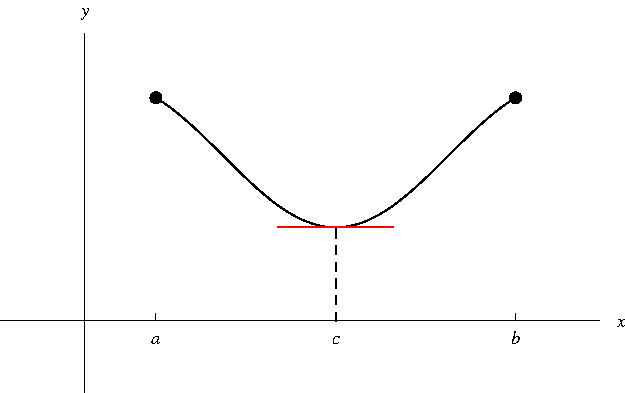
\includegraphics[height=2.5cm]{maxima-minima/pictures/04-02-rollesd.pdf}%
\column{.6\textwidth}
\begin{enumerate}
\setcounter{enumi}{2}
\item  $f(x) < f(a)$ for some $x$ in $(a,b)$.
\end{enumerate}
\begin{itemize}
\item<2->  By the Extreme Value Theorem, $f$ has a minimum in $[a,b]$.
\item<3->  Since $f(x) < f(a)$, this value is attained at some $c$ in $(a,b)$.
\item<4->  \alert<handout:0| 4>{Fermat's Theorem}: $f'(c) = 0$.\qedhere
\end{itemize}
\end{columns}
\end{proof}

\vspace{2cm} %guarantees top alignment of slide
\end{frame}
% end module rolles-theorem
